% !TeX root = ../../ZF_bmicha_Ana.tex
\subsection{Gradient}
    \vspace{-0.75em}
    $$
        \grad(f(x,y,z)) = 
        \begin{pmatrix}
            f_x \\ f_y \\ f_z
        \end{pmatrix}
        =
        \begin{pmatrix}
            \frac{\partial}{\partial x} \\[0.4em] \frac{\partial}{\partial y} \\[0.4em] \frac{\partial}{\partial z}
        \end{pmatrix}
    $$
    \begin{itemize}
        \item Steht senkrecht auf Niveauflächen/ -linien.
        \item Zeigt in Richtung des grössten Anstiegs der Funktionswerte.
    \end{itemize}
    \vspace*{0.5em}
    \subsubsection{2D - $f(x,y)$}
        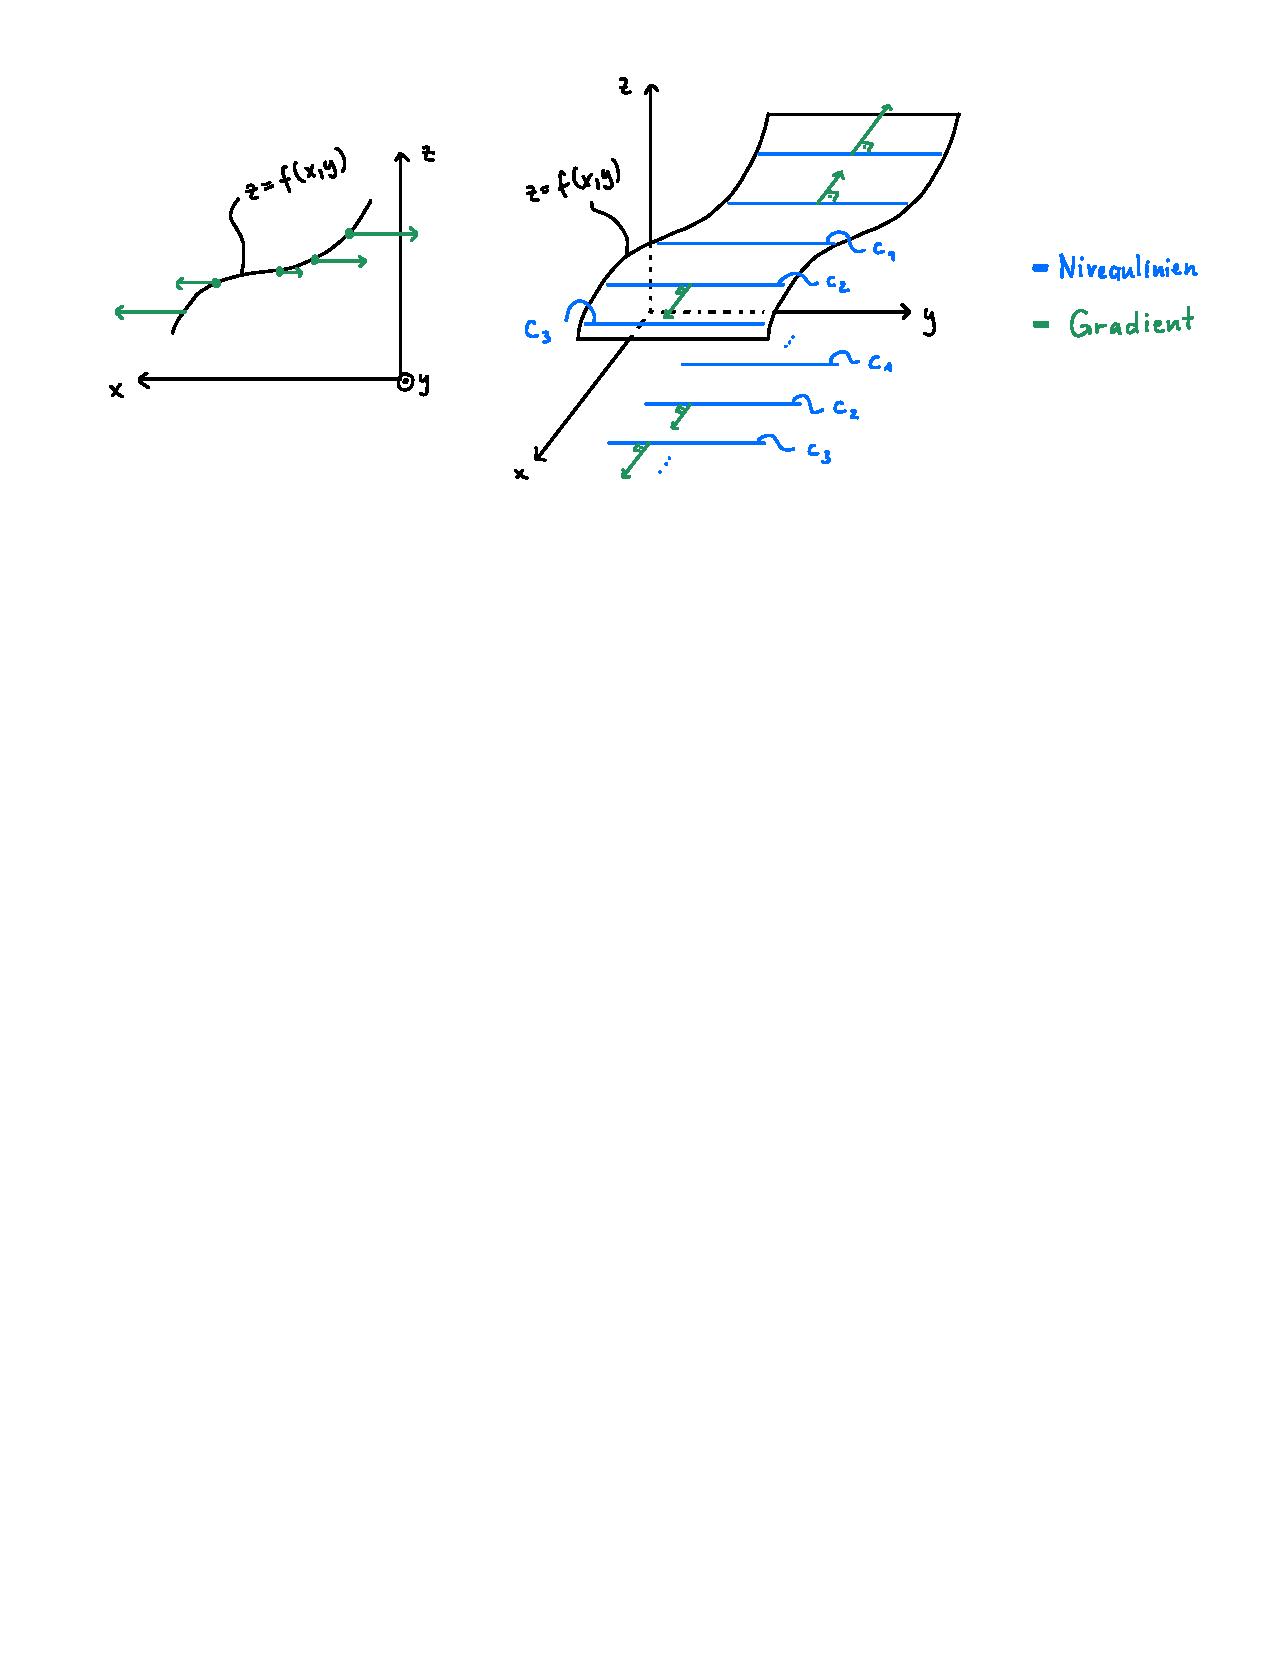
\includegraphics[width=\linewidth]{src/Mehrdimensionale-Funktionen_Differentialrechnung/grad_2D.pdf}
    \subsubsection{3D - $f(x,y,z)$}
        \begin{center}
            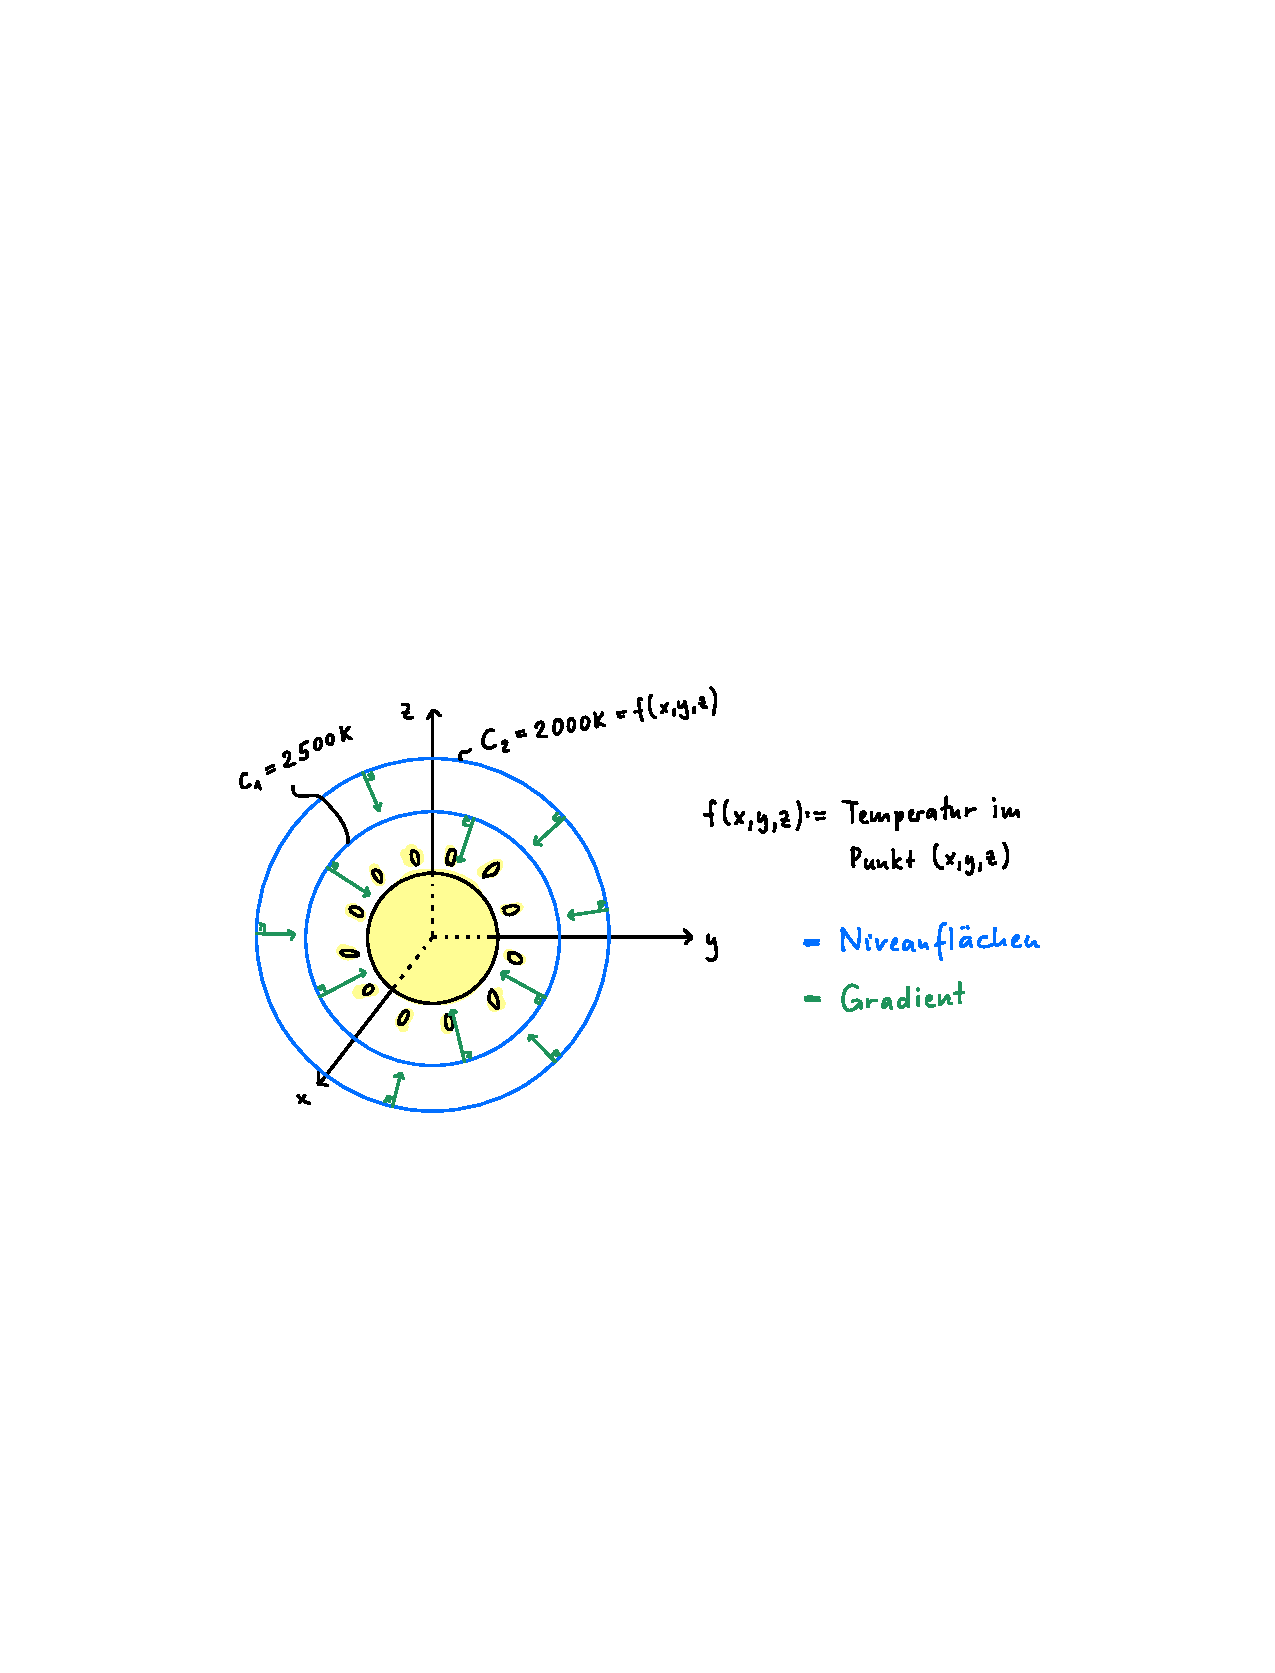
\includegraphics[width=0.8\linewidth]{src/Mehrdimensionale-Funktionen_Differentialrechnung/grad_3D.pdf}
        \end{center}